\chapter{How to obtain the CRTM}
%===============================

\section{CRTM ftp download site}
%===============================
The CRTM source code and coefficients, and example programs, are released as compressed tarballs\footnote{A compressed (e.g. gzip'd) tape archive (tar) file.} via the CRTM ftp site:

\hspace{1cm}\texttt{ftp://ftp.emc.ncep.noaa.gov/jcsda/CRTM/}

A snapshot of that site is shown in figure \ref{fig:ftp_site}. Note that the source code and coefficients can be released separately as updates to either one can occur independently of the other. Also note that additional releases, e.g. beta or experimental branches, are also made available on this ftp site.

\begin{figure}[htb]
  \centering
  \includegraphics[scale=0.5]{graphics/Get/CRTM_ftp_site.eps}
  \caption{The CRTM ftp site contents (as on Mar.12, 2010)}
  \label{fig:ftp_site}
\end{figure}

\section{Coefficient Data}
%=========================
The tarball labeled as ``\texttt{Coeffs}'' packages up all the transmittance, spectral, cloud, aerosol, and emissivity coefficient data needed by the CRTM. The coefficient tarball directory structure is organised by coefficient and format type as shown in figure \ref{fig:crtm_coefficients_dir}.

\begin{figure}[htb]
  \centering
  \input{graphics/Get/CRTM_Coefficients_dir.pstex_t}
  \caption{The CRTM coefficients tarball structure}
  \label{fig:crtm_coefficients_dir}
\end{figure}

Both big- and little-endian format files are provided to save users the trouble of switching what they use for their system. Note in the TauCoeff directory there are two subdirectories: ODAS and ODPS. These directories correspond to the coefficient files for the different transmittance model algorithms. The user can select which algorithm to use by using the corresponding TauCoeff file.

To run the CRTM, all the required coefficient files need to be in the same path (see the  \hyperref[sec:CRTM_Init_interface]{CRTM initialisation function} description) so users will have to move/link the datafiles as required.


\section{Example Programs}
%=========================
The tarball labeled as ``\texttt{Example\_Code}'' contains two completely independent sets of example programs -- one showing how to call the CRTM Forward model and the other for the K-matrix model. The Example Code tarball directory structure is shown in figure \ref{fig:example_code_dir}  where the directories for each example program are highlighted in blue, and shell scripts to run them are shown in red.

\begin{figure}[htb]
  \centering
  \input{graphics/Get/Example_Code_dir.pstex_t}
  \caption{The example code tarball structure. The example programs are shown in blue, and shell scripts to run them are shown in red.}
  \label{fig:example_code_dir}
\end{figure}

Some notes about building the example programs:
\begin{itemize}
  \item The shell script files, \texttt{run\_Example\_Forward.sh} and \texttt{run\_Example\_K\_Matrix.sh}, both build and run the example programs which include a comparison of their output to that supplied in the \texttt{Results} directory.
  \item The \texttt{makefile.common} file contains all the relevant macro definitions for the compilation. This file should be modified by users to alter the various macros and compilers flags to accomodate their system.  This file uses the \texttt{FC} and \texttt{FC\_FLAGS} macros to define the Fortran95 compiler and switches respectively. Currently the default compiler is \texttt{gfortran}, but additional definitions for different compilers are provided at the bottom of the file. Similarly for the \texttt{FL} and \texttt{FL\_FLAGS} macro definitions.
  \item it is assumed the CRTM library has already been built (see chapter \ref{sec:build} for how to do that) \emph{and} is in the generic location defined by the \texttt{CRTM\_DIR} macro (currently setup for our JCSDA systems.)
\end{itemize}
You should modify the \texttt{makefile.common} file for your own system. As mentioned, other compiler switches are provided for guidance. 




